\documentclass[11pt,a5paper]{article}

\usepackage[T1]{fontenc}
\usepackage[utf8]{inputenc}
\usepackage{lmodern, microtype}
\usepackage[estonian]{babel}
\usepackage{siunitx}
\sisetup{inter-unit-product=\ensuremath{{}\cdot{}}, per-mode=fraction, exponent-product=\cdot, output-decimal-marker={,}, uncertainty-mode=separate}
\usepackage{graphicx}
\usepackage{wrapfig}
\usepackage{tikz}
\usetikzlibrary{arrows.meta, patterns, patterns.meta}
\usepackage[european]{circuitikz}
\usepackage{pgfplots}
\tikzset{component/.style={draw,thick,circle,fill=white,minimum size=0.75cm,inner sep=0pt}}
\usepackage{amsmath,amssymb,amsfonts}
\usepackage[hidelinks]{hyperref}
\usepackage{csquotes}
\usepackage{caption}
\usepackage{enumitem}
\topmargin=-3.0cm \textheight=19cm \textwidth=12.9cm
\oddsidemargin=-1.5cm  \evensidemargin=-1.5cm
\setlength{\parindent}{0pt} \setlength{\parskip}{6pt} \sloppy
\sloppy \relpenalty=10000 \binoppenalty=10000
\pagestyle{empty}


\newcommand{\numb}[1]{\vspace{5pt}\textbf{\large #1}}
\newcommand{\nimi}[1]{(\textsl{\small #1})}
\newcommand{\punktid}[1]{(\emph{#1~p.})}
\newcommand{\p}[1]{[\textbf{#1~p}]}
\newcounter{ylesanne}
\newcommand{\yl}[1]{\addtocounter{ylesanne}{1}\numb{\theylesanne.} \nimi{#1} \newblock{}}
%\newcommand{\autor}[1]{}% Kasuta võistluse ajal
\newcommand{\autor}[1]{\emph{Autor: #1}}% Kasuta kui vaja autorit
\newcommand{\autorl}[1]{\emph{Lahenduse autor: #1}}% Kasuta kui vaja autorit



\begin{document}
\normalsize
\begin{center}
  \textbf{\Large Eesti koolinoorte 69.\ füüsikaolümpiaad} \par
  \emph{12.\ veebruar 2022. a.\\ \textbf{Gümnaasiumi} ülesannete lahendused (10.--12.\ klass)}
\end{center}

\normalsize

\numb{Eessõna}

Allpool on toodud iga ülesande üks õige lahenduskäik (mõnel juhul ka enam). \textbf{Kõik alternatiivsed õiged lahenduskäigud tuleb hinnata samuti maksimumpunktidega.} Iga alternatiivse lahenduskäigu jaoks tuleb kontrollijatel koostada hindamisskeem, juhindudes võimalusel juuresoleva hindamisskeemi punktijagamisproportsioonist. Soovituslikud maha-arvamise punktid:

\yl{PEEGEL PEEGLIS}
\punktid{6} \autor{Richard Luhtaru}

Konstrueerime Arvo kujutise peeglis 1 ($A'$), peeglis 2 ($A''$) ja punkti $A'$ kujutise peeglis 2 ($A'''$). Breti nägemiseks on kaks võimalust. Esimene võimalus on ainult peegli 1 kaudu, kiirte käigu saame konstrueerida lõigu $A'B$ abil. Teine võimalus on peegli 1 ja seejärel peegli 2 kaudu, kiirte käigu saame konstrueerida lõigu $A'''B$ abil. Ainult peeglist 2 pole võimalik Bretti näha, sest $A''B$ ei lõiku peegliga 2. Samuti pole peeglist 2 võimalik näha peeglit 1, seega rohkem võimalusi pole.

\begin{figure}[h]
    \centering
    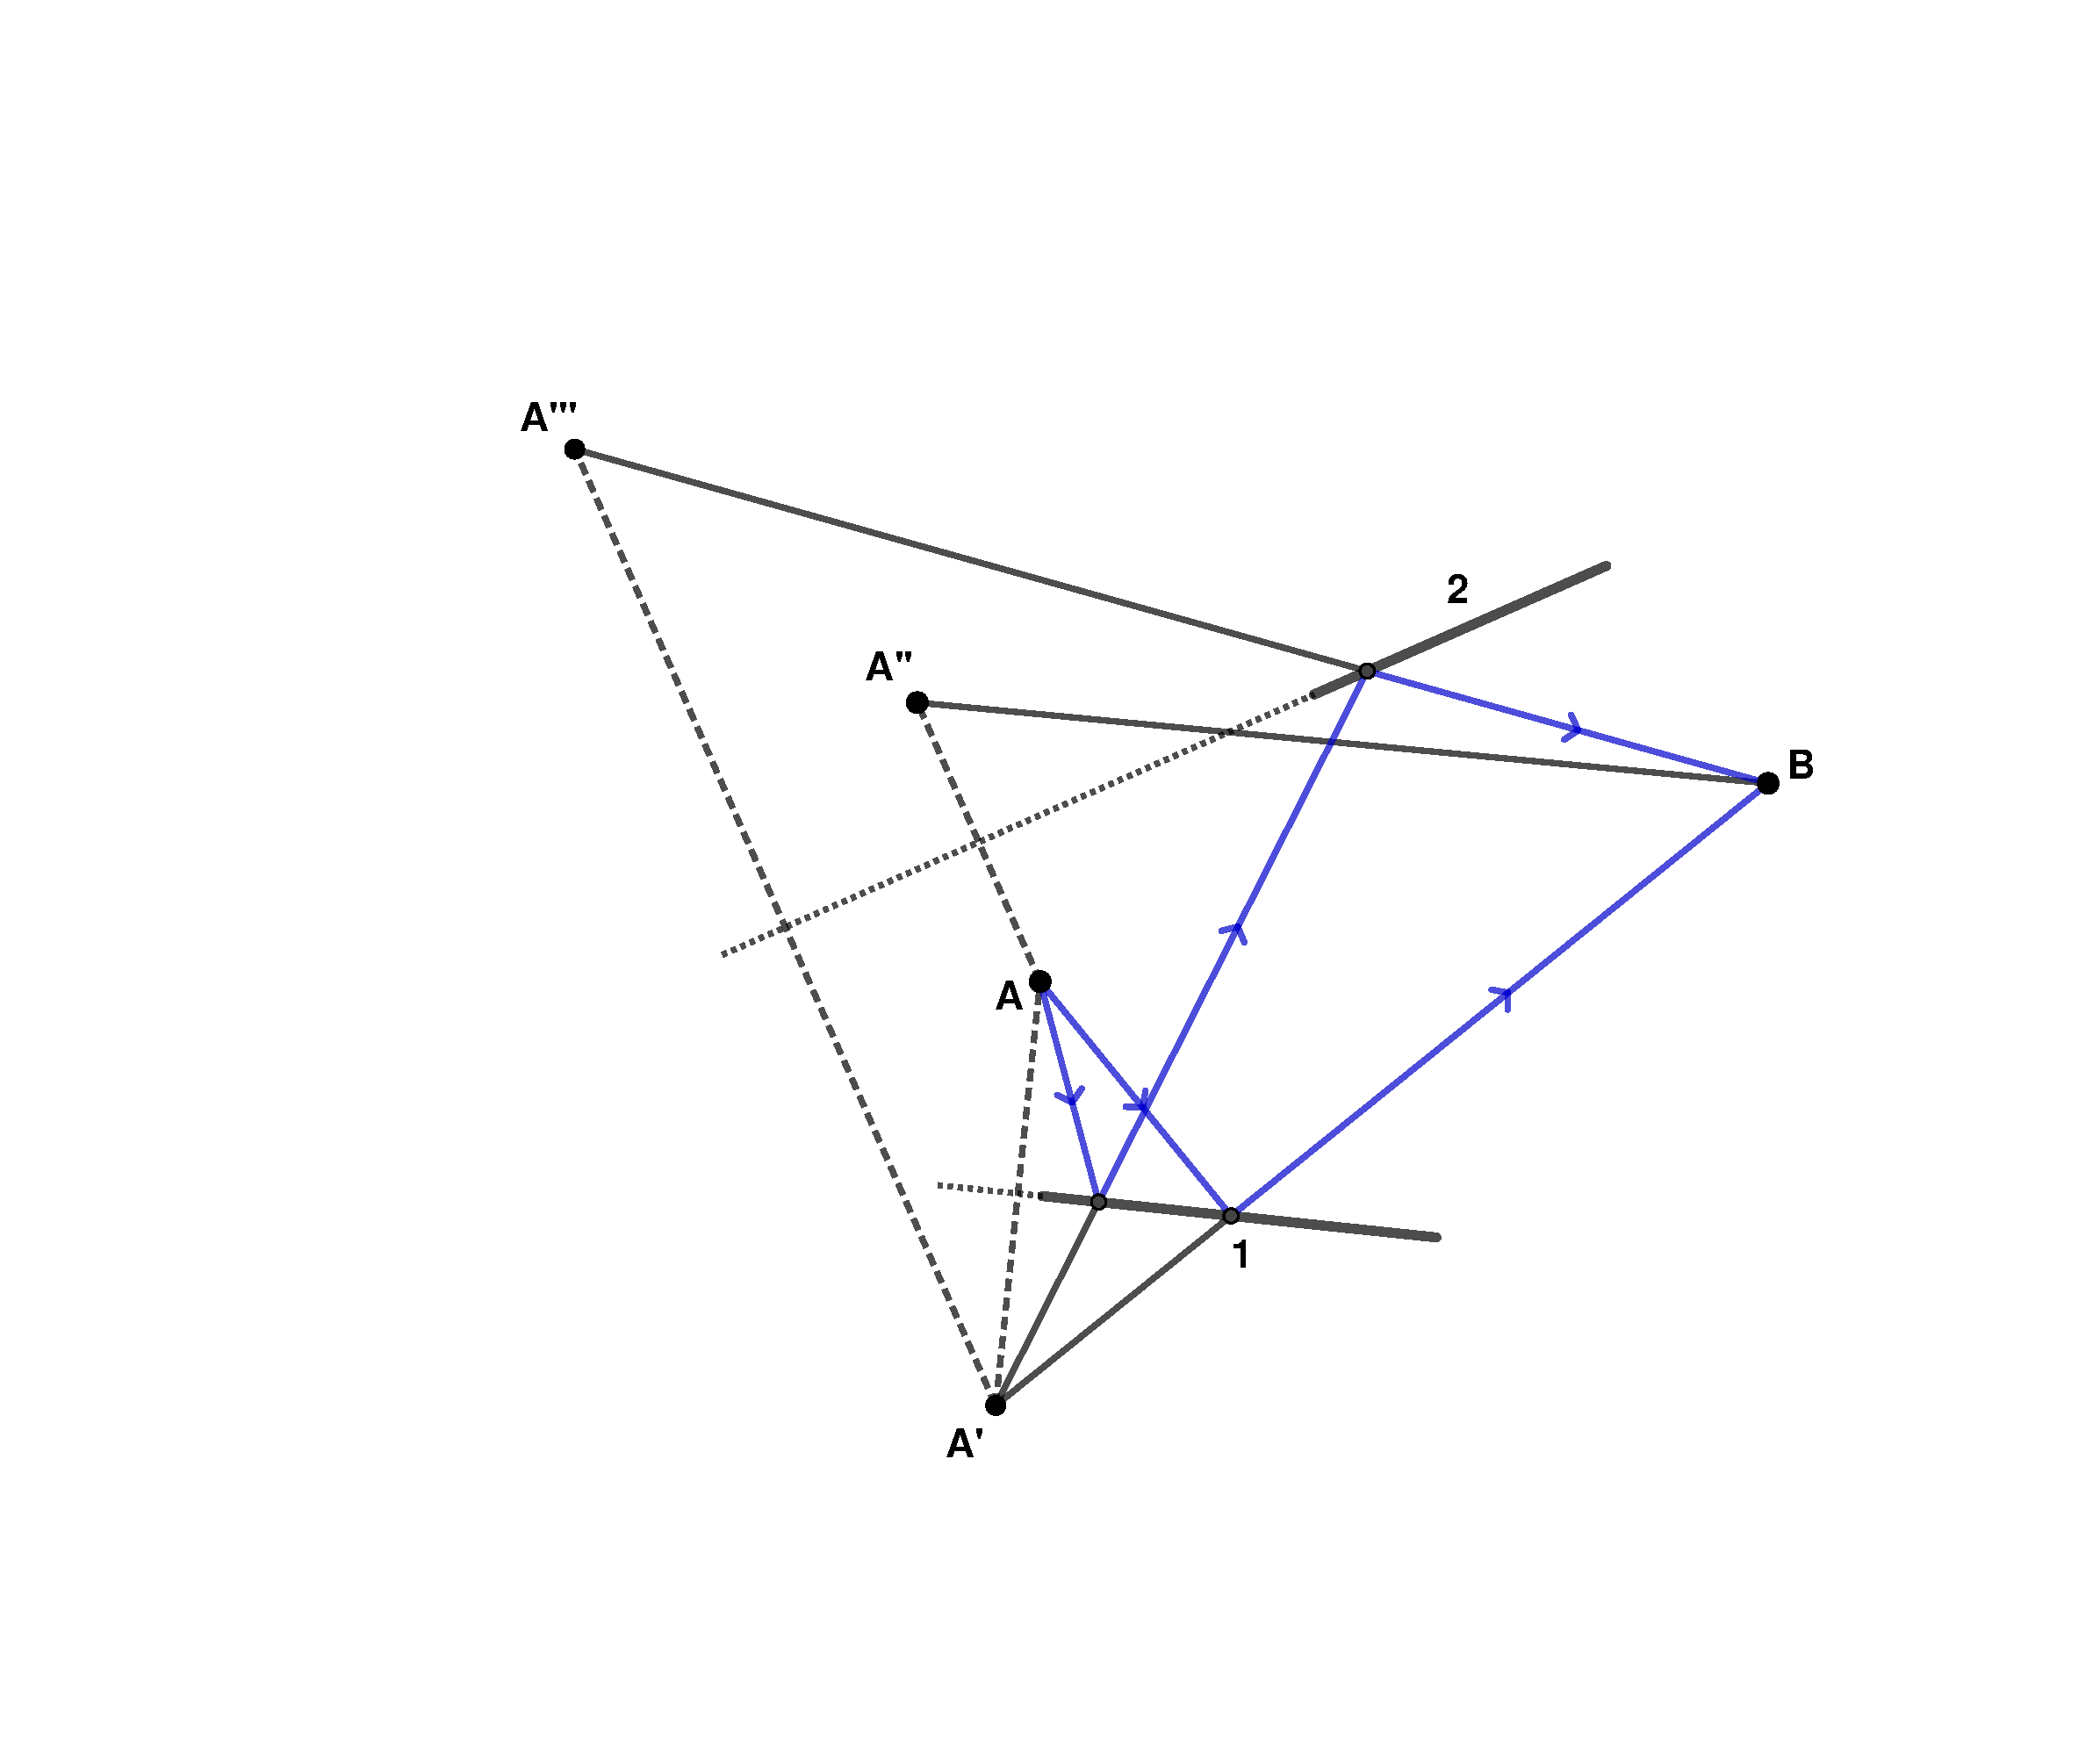
\includegraphics[width=\textwidth, trim=0 50 0 50, clip]{spiegel_lah_joonis}
\end{figure}

\newpage
\yl{JUHE}
\punktid{8} \autor{Jaan Kalda}

$P=V_0^2/R$, millest $R=V_0^2/P=\qty{26.45}{\ohm}$. Leiame vasktraadist juhtme takistuse $r=2L\rho/S=\qty{1.36}{\ohm}$. Vool juhtmes $I=V_p/(R+r)=\qty{8.6}{\A}$ ning juhtmes eralduv võimsus $P_j=rI^2=rV_p^2/(R+r)^2\approx\qty{101}{\W}$.

\newpage
\yl{LIUMÄGI}
\punktid{8} \autor{Kaarel Kivisalu}

\emph{Lahendus 1}:
Kalpinna pikkus on $h/\sin \alpha$ \p{0,5}. Horisontaalse pinna pikkus on $l-h/\tan \alpha$ \p{0,5}.
Hõõrdejõud kaldpinnast alla lastes on $F=\mu g \cos \alpha$ \p2. Energia jäävus (potentsiaalse energia muut on võrdne hõõrdejõu tööga):
\begin{equation*}
mgh = \mu mg \cos \alpha \cdot \frac{h}{\sin \alpha} + \mu mg \cdot \left(l- \frac{h}{\tan \alpha}\right). \quad \p4
\end{equation*}
Järelikult $\mu=h/l$ \p1.

\emph{Lahendus 2}:
Kiirendus kaldpinnast alla lastes on $a_1=g \sin \alpha - \mu g \cos \alpha$ \p2. Kalpinna pikkus on $h/\sin \alpha$ \p{0,5}. Järelikult kiirus kaldpinna lõpus on
\begin{equation*}
  v=\sqrt{\frac{2a_1h}{\sin \alpha}}. \quad \p{1,5}
\end{equation*}
Horisontaalse pinna pikkus on $l-h/\tan \alpha$ \p{0,5}. Kuna üleminek kaldpinnalt horisontaalsele pinnale on sujuv, siis kiirus ei muutu. Kiirendus horisontaalsel pinnal on $a_2= - \mu g $. Kuna liumäe lõpus peab alla lastes seisma jääma, siis
\begin{equation*}
  v=\sqrt{-2a_2\left(l-\frac{h}{\tan \alpha}\right)}.\quad \p{1,5}
\end{equation*}
Järelikult
\begin{equation*}
  2\mu g\left(l-\frac{h}{\tan \alpha}\right)=\frac{2h(g\sin \alpha - \mu g \cos \alpha)}{\sin \alpha}, \quad \p1
\end{equation*}
võrrantit lihtsustades saame, et $\mu=h/l$ \p1.

\yl{KAKS TUBA}
\punktid{8} \autor{Jarl Patrick Paide}

Olgu mõlemas toas algne kütteallikas võimsusega $N$ \p{0,5}. Olgu toas, kus on lisaks kütteallikas võimsusega $P$ temperatuur $T_0$, teises toas temperatuur $T_1$ ja väljas temperatuur $T_2$. Süsteem on tasakaalus kui $T_0 > T_1 > T_2$ \p{0,5}. Paneme kirja võrrandi mõlema toa jaoks kus paremal pool on toast lahkuv soojus ja vasakul pool tuppa sisenev soojus.
\begin{align*}
  N+P&=3k(T_0 - T_2)+k(T_0-T_1), \quad \p2\\
  N+k(T_0-T_1)&=3k(T_1 - T_2). \quad \p2
\end{align*}
Siit saame avaldada temperatuurivahe $T_0-T_1=\frac{P}{5k}$ \p3.

\newpage
\yl{SATELLIITTELEVISIOON}
\punktid{8} \autor{Krister Kasemaa}

Leiame geostatsionaarse orbiidi raadiuse. Sateliidile mõjuvad jõud on tasakaalus:
\begin{align*}
\frac{GMm}{r_\text{orbiit}^2}&=\frac{mv^2}{r_\text{orbiit}}\\
\implies \frac{GM}{r_\text{orbiit}}&= \bigg( \frac{2\pi r_\text{orbiit}}{T} \bigg)^2\\
\implies r_\text{orbiit}^3 &= T^2 \frac{GM}{4 \pi^2}.
\end{align*}
Maakera pinnal aga kehtib mingi suvalise massi $m$ jaoks:
\begin{equation*}
  \begin{cases}
    F = \frac{GMm}{R_\oplus^2}, \\
    F = mg. \\
  \end{cases}
\end{equation*}
Seega, $GM = g R_\oplus^2$. Asendades saadud seose orbiidi raadiuse valemisse, saame:
\begin{align*}
r_\mathrm{orbiit}^3 &= T^2 \frac{g R_\oplus^2}{4 \pi^2},\\
\implies r_\mathrm{orbiit} &\approx \SI{42148}{km}.
\end{align*}
Maksimaalsel sateliittelevisiooni võimaldaval laiuskraadil on sateliiti ja maakera ühendav sirge maakera puutujaks sellel maksimaalsel laiuskraadil. Seega saame seose:
\begin{figure}[h]
  \centering
  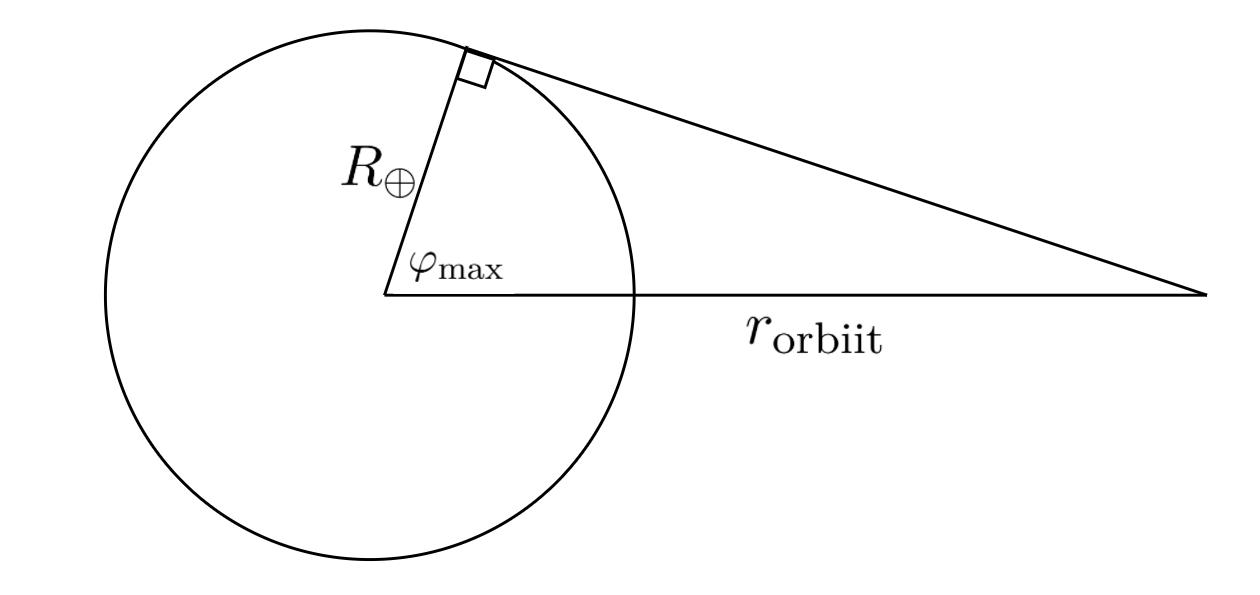
\includegraphics[width = 0.7\textwidth]{satteliittelevisioon_diagramm.png}
\end{figure}
\begin{equation*}
\varphi_\mathrm{max} = \arccos{\left( \frac{R_\oplus}{r_\text{orbiit}}\right)} = \ang{81.3}
\end{equation*}

\yl{DOOMINO}
\punktid{8} \autor{Päivo Simson}

\begin{equation*}
\tau=\frac{d}{u}. \qquad \p1
\end{equation*}
Sellel hetkel peab kuulike olema kõrgemal kui doominoklotsi kõrgus $h$, et mitte klotsi ümber lükata. Vähimale kiirusele vastab pikim võimalik liikumise aeg \p1. On selge, et selleks peab kuulike pärast põrget uuesti tõusma kõrgusele $H$ ja seejärel langema klotsini jõudmise hetkeks mitte madalamale kui $h$ \p1. Kõrguselt $H$ kukkumise aja $t_1$ saame leida seosest $H=gt_1^2/2$, mis annab
\begin{equation*}
t_1=\sqrt{\frac{2H}{g}}. \qquad \p1
\end{equation*}
Sama aeg kulub ka pärast põrget uuesti kõrgusele $H$ tõusmiseks. Kõrguselt $H$ kõrgusele $h$ langemiseks kulub aeg
\begin{equation*}
t_2=\sqrt{\frac{2(H-h)}{g}}. \qquad \p1
\end{equation*}
Kokku kulub klotsi ülemise servani jõudmiseks aeg $2t_1+t_2=\tau=d/u$ \p1. Siit saame pärast lihtsustamist minimaalseks kiiruseks
\begin{equation*}
  u=\frac{d\sqrt{g}}{2\sqrt{2H}+\sqrt{2(H-h)}}. \qquad \p1
\end{equation*}

\newpage
\yl{PLASTILIIN}
\punktid{10} \autor{Taavet Kalda}

Peale esimest kokkupõrget nihkub plaadi tasakaaluasend $mg/k$ võrra allapoole ning plaat hakkab uue tasakaaluasendi ümber teatud amplituudiga võnkuma (amplituudi väärtust pole punktide saamiseks vaja leida) \p3. Kuna plaadi mass on plastiliini massiga võrreldes tühine, omandab plaat kokkupõrke hetkel impulsi jäävuse tõttu sama kiiruse nagu plastiliin, seega plaadi kiirus on energia jäävusest $v_0 = \sqrt{2gh}$ ($v_0$ avaldist pole punktide saamiseks vaja leida). Energia jäävusest järeldame, et plaadi kiirus on samuti $v_0$ siis, kui teine plastiliinitükk plaadiga kontakti loob \p2. See tuleneb asjaolust et plaadi kõrgus lauast, ehk teisisõnu plaadi potentsiaalne energia, on hetk enne teist kokkupõrget sama mis see oli just peale esimest kokkupõrget. Seega on teise plastiliini kokkupõrge plaadiga efektiivselt sama kui kahe identse massi ja kiirusega objektide lauskokkupõrge. Seega jääb plaat peale teist kokkupõrget seisma \p2. Samas nihkub plaadi tasakaaluasend veel $mg/k$ võrra allapoole ning plaat hakkab amplituudiga $2mg/k$ uue tasakaaluasendi ümber võnkuma \p2. Seega on järgneva liikumise käigus plaadi kõige alumine asend $4mg/k$ võrra esialgsest asendist all pool \p1.

\yl{TÜHI PUDEL}
\punktid{10} \autor{Jaan Kalda}

Rõhk pudelis kasvab kahel põhjusel. Esiteks, toimub pudelisse suletud õhu (va veeauru molekulid) isohooriline paisumine toatemperatuurilt kuni vee tempreatuurini --- võime eeldada, et raputamise käigus annab vesi soojust õhule ning vee soojusmahtuvus on nii suur, et see ei jõua oluliselt jahtuda \p1. Teiseks kasvab õhus veeauru osarõhk, korraliku raputamise tulemusel saabub pudelisse termodünaamiline tasakaal, mis tähendab, et pudelis oleva õhu temperatuur võrdub vee temperatuuriga ja veeauru rõhk võrdub küllastunud auru rõhuga antud temperatuuril \p1.

Esimese komponendi leidmiseks paneme tähele, et enne raputamist oli õhu osarõhk pudelis (õhu rõhk ilma veeauru rõhuta) $p_0'=p_0-rp_k(\qty{20}\celsius)\approx p_0$, sest veeauru osarõhk on palju väiksem atmosfäärirõhust. Avaldis õhu osarõhu jaoks pudelis enne loksutamist, olgu see siis täpne või lihtsustatult $p_0$, annab \p1; selle punkti saab kätte ka siis, kui õpilane kasutab ilma pikemalt põhjendamata järgnevas isohoori seaduses atmosfäärirõhku $p_0$). Eelnevas avaldises esines auru rõhu osarõhk toaõhus $p_a=rp_k(\qty{20}\celsius)$ \p1, mille väärtust läheb hiljem vaja.  Selle arvuliseks leidmiseks tuleb võtta graafikult lugem küllastunud auru rõhu jaoks, $p_k(\qty{20}\celsius)\approx \qty{2.2}{\kPa}$; täpne lugem (väärtused vahemikus $\qty{2.2\pm 0.1}{\kPa}$) annab \p1 ja vähem täpne lugem (väärtused vahemikus $\qty{2.2\pm 0.2}{\kPa}$) annab \p{0,5} (suurema vea korral punkte ei saa). Ideaalse gaasi olekuvõrrandist teame, et konstantsel ruumalal on rõhk võrdeline temperatuuriga, seega uus õhu osarõhk $p_1= p_0T_v/T_t$ \p1 ning järelikult vastav rõhu kasv pudeli sees $\Delta p_1\equiv p_1-p_0=p_0'(T_v/T_t-1)\approx \SI{12}{\kPa}$ (avaldis $\Delta p_1$ jaoks annab \p1 ja õige numbriline väärtus \p1), kus temperatuurid on esitatud Kelvinites.

Teise komponendi leiame kui veeauru rõhkude vahe: $\Delta p_2 = p_k(\qty{55}{\celsius}) - \num{0.5}p_k(\qty{20}{\celsius}) \approx \SI{15}{\kPa} -\num{0.5}\cdot\qty{2.2}{\kPa}\approx \qty{14}{\kPa}$. Idee eest avaldada veeauru osarõhu muutus graafikult loetavate rõhkude vahena annab \p1; $p_k(\SI{55}\celsius)$ korrektne leidmine graafikult (väärtused vahemikus $\SI{1.5\pm 0.1}{kPa}$)  annab veel \p1 (suurema vea korral saab vahemiku $\SI{1.5\pm 0.2}{kPa}$ korral \p{0,5}).

Seega oli rõhk pudelis $\approx \SI{25}{kPa}$ võrra suurem, kui toas.

\yl{PIKNE}
\punktid{12} \autor{Jaan Kalda}

\osa Elektriväli maapinnal on elektriväli plaatkondensaatori sees, seega $E=Q/\varepsilon_0S$, kus $S$ on plaadi (st pilve alumise pinna) pindala \p3. Selle avaldise võib leida Gaussi seadusest võrrutades elektrilise $D$-välja voo $ES/\varepsilon_0$ mõttelise pinna sisse jääva laenguga $Q$. Alternatiivselt võib selle leida plaatkondensaatori mahtuvuse valemist, mispuhul jagunevad need 3 punkti järgnevateks tükkideks: mahtuvuse $C$ definitsiooni $q=UC$ eest (suvalisel ekvivalentsel kujul) \p1; elektrivälja tugevuse ja pinge vahelise seose $U=Ed$ eest \p1; valemi $C=\varepsilon_0S/d$ eest \p1. Siit avaldame pilve kogulaengu $Q=\varepsilon_0E\pi d^2/4\approx\SI{80}C$ (valemi eest \p1). Välguna maha voolanud laengu leiame kui keskmise voolutugevuse ja vooluimpulsi kestvuse korrutise, $q=I\tau=\SI{30}C$ (avaldise eest \p1). Seega maha voolas $300/8\%\approx 40\%$ kogulaengust; õige numbrilise vastuse eest \p1.

\osa Vaatleme mõttelist poolsfääri maa sees raadiusega $r$: vool $I$ jaguneb ühtlaselt üle selle pinna nii, et voolu ruumtihedus $j=I/2\pi r^2$ \p2. Sellisel juhul elektrivälja tugevus $E=\rho j$ \p1, seega $E=I\rho/2\pi r^2$ ning jalgade vahele jääv pinge $U=Eh$ \p1, millest saame asendamiste järel $U=I\rho h/2\pi r^2$, kus $h\approx\SI 1m$ tähistab jalgade vahemaad (mõistliku hinnangu tegemine \num{0.5} meetrist \num{1.2} meetrini annab \p1). Seega kaugus välgulöögi kohast $r=\sqrt{I\rho h/2\pi U}\approx\SI{52}m$; õige arvuline väärtus, mis vastab kasutatud $h$ väärtusele annab \p1 .
\\\emph{Märkus:} lihtsa valemi $U=Eh$ asemel võib kasutada ka integreerimist, $U=\int_r^{r+h} E\textrm dr=I\rho h/2\pi[1/r-1/(r+h)]$, aga selline täpsus pole vajalik, sest jalgade vahelise vahemaa pikkus ise on palju ebatäpsem, kui saavutatud võit täpsuses, seetõttu selline integreerimine punkte juurde ei anna.

\newpage
\yl{PINGPONG}
\punktid{12} \autor{Jaan Kalda}

\emph{Märkus}: graafikult numbrite välja lugemise eest antakse punkte isegi siis, kui õpilane ei oska nendega midagi peale hakata.

\osa Teeme kindlaks esimese kuue põrke hetked sekundites: \num{0,92}; \num{1,93}; \num{2,78}; \num{3,49}; \num{4,1}; \num{4.61} (\p1; punkti teenimiseks piisab, kui välja on loetud esimesed kaks ja viimased kaks andmepunkti; kui on välja loetud vähem, kui neli andmepunkti, siis punkte ei anta; kui välja loetud andmepunktid ei sisalda esimest või kuuendat põrget, siis antakse \p{0,5}). Kuigi samplimise sagedus on $\SI{0.1}s$, siis graafikult on näha, et tulemusi saab välja lugeda täpsemalt --- ilmselt on graafikuid interpoleeritud (seda hindamisskeem ka eeldab: punkte ei alandata, kui välja loetud arvväärtused erinevad eeltoodutest mitte rohkem, kui $\SI{0.02}s$ võrra; kui ühes andmepunktis on suurem viga, mis pole siiski rohkem, kui  $\SI {0.04}s$, siis alandatakse skoori \p{0,5} võrra ja kui vigade arv on suurem, siis punkte ei anta).

Nende põhjal saame arvutada esimesele viiele põrkele järgnenud lennuajad sekundites: \num{1,01}; \num{0,85}; \num{0,71}; \num{0,61}; \num{0,51} (\p1; kui esimeses või viimases arvus on viga suurem, kui $\SI {0.03}s$, siis alandatakse skoori \p{0,5} võrra ja kui see on suurem, kui $\SI{0.05}s$, siis punkte ei anta).

Ülesande eelduste kohaselt peaks vähenema kineetiline energia geomeetrilise jadana: $T_n=mv_n^2/2=T_0k^n$ (valemina kirja panemise eest \p1). Kiirus $v_n$ on võrdeline ruutjuurega energiast, seega $v_n=v_0\sqrt{k^n}$ \p1 ning lennuaeg $t_n=2v_n/g$ on võrdeline kiirusega, seega $t_n=t_0\sqrt{k^n}$ \p1. Mõõdetud andmete kasutamise parim meetod oleks kanda need graafikule, kus horisontaalteljel on põrkenumber ja vertikaalteljel --- lennuaja logaritm $\ln t_n=\ln t_0 + \frac 12n\ln k$:  ning nimetatud teljestikus peaks tulema sirgjoon, mille kahekordne tõusunurga tangens annaks meile $\ln k$ väärtuse. Aga hea tulemuse saame ka, kui võtame viienda ja esimese lennuaja suhtest ruutjuure:  $k=\sqrt{0.51/1.01}\approx 0.71$, mis tähendab, et 29\% kineetilisest energiast kaob igal põrkel (ükskõik kumma meetodi rakendamine annab \p1). Õige numbrilise vastuse eest (vahemikus 25\% kuni 35\%) saab \p1, ebatäpse vastuse eest (vahemikus 20\% kuni 40\%) saab pooled punktid, st \p{0,5}. NB! Arvulise väärtuse eest saab punkte vaid siis, kui see tuleneb õige meetodi rakendamisest.

\osa Alates üheksandast põrkest on põrkeajad nii väiksed, et eelpooltoodud arvutuste läbiviimine on küll võimalik, kuid ebatäpne; kui viiakse läbi selline analüüs, siis saab selle ülesande osa (b) eest vaid kuni \p2: vastuse eest vastavalt allpooltoodud reeglile kuni \p1 ning kuni \p1 graafikult põrkehetkede välja lugemise eest (kui kasvõi ühes arvutusteks vajalikus andmes on viga suurem, kui $\SI{0.02}s$, siis \p{0,5} ning kui see on suurem, kui $\SI{0.04}s$, siis \p0).

Selle asemel kasutame teist meetodit: kuivõrd põrkeaegadest moodustub geomeetriline jada, siis palli seismajäämise hetke saab avaldada geomeetrilise jada summana. Kaheteistkümnes põrge toimub ajahetkel $\SI{6.97}s$ ja järgmine põrge --- ajahetkel $\SI{7.27}s$ (mõlemad andmepunktid kokku \p1; kui kasvõi ühes neist on viga suurem, kui $\SI {0.02}s$, siis alandatakse skoori \p{0,5} võrra ja kui see on suurem, kui $\SI {0.04}s$, siis punkte ei anta) ning põrked lõppevad ajahetkel $\SI{12.3}s$ (\p1; kui viga on suurem, kui $\SI {0.02}s$, siis alandatakse skoori \p{0,5} võrra ja kui see on suurem, kui $\SI {0.04}s$, siis punkte ei anta). Siit saame leida kaheteistkümnenda põrke kestvuse $t_{12}=\SI{0.3}s$.
Mõõtes nüüd ajavahemiku kaheteistkümnendast põrkest põrkumiste lõpuni $T=t_{12}/(1-\sqrt k)=\SI{5.33}s$ \p1 on lihtne leida $k=(1-t_{12}/T)^2\approx 0.88$ \p1, mis tähendab, et igal põrkel kaob 12\% kineetilisest energiat \p1. Kui vastus erineb antud numbrist rohkem, kui 1\% võrra, siis saab numbrilise vastuse eest vaid \p{0,5} punkti ning kui see erineb rohkem, kui 2\% võrra, siis punkte ei saa.

\emph{Märkus:} Tasub tähele panna, et saadud tulemus pole väga täpne, sest samplimise sagedus on ju vaid $\SI{0.1}s$, mistõttu $t_{12}$ leidmise suhteline viga on võrdlemisi suur. Seetõttu on täpsemateks arvutusteks vaja kasutada ka järgnevaid andmepunkte (põrgete hetked $\SI{7.58}s$, $\SI{7.88}s$, $\SI{8.17}s$ ja $\SI{8.39}s$) ning keskmistada. Geomeetrilises jadas on jada keskmine liige kõigi liikmete geomeetriline keskmine, aga kui keskmistatavad arvud erinevad üksteisest vähe, siis on geomeetriline keskmine ligikaudu võrdne aritmeetilise keskmisega. Seega me võime leida $t_{14}=(\num{8.39}-\num{6.97})\unit{s}/5= \SI{0.284}s$. Arvutades nüüd juba ajavahemiku neljateistkümnendast põrkest põrkumiste lõpuni $T'=t_{14}/(1-\sqrt k)=\SI{4.72}s$, saame tulemuseks $k=(1-t_{14}/T')^2\approx 0.88$, mis osutus võrdseks me esialgse tulemusega.


\end{document}